\documentclass[11pt,a4paper]{article}
\usepackage[utf8]{inputenc}
\usepackage[T1]{fontenc}
\usepackage[margin=1in]{geometry}
\usepackage{amsmath}
\usepackage{xcolor}
\usepackage{graphicx}
\usepackage{booktabs}
\usepackage{tabularx}
\usepackage{enumitem}
\usepackage{titlesec}
\usepackage{fancyhdr}
\usepackage{hyperref}
\usepackage{listings}
\usepackage{float}

% Colors
\definecolor{accent}{HTML}{2C3E50}
\definecolor{codeblue}{HTML}{2980B9}
\definecolor{codegray}{HTML}{7F8C8D}
\definecolor{lightgray}{HTML}{F5F5F5}

% Section styling
\titleformat{\section}{\large\bfseries\color{accent}}{\thesection.}{0.5em}{}[\vspace{-0.3em}\textcolor{accent}{\rule{\textwidth}{0.5pt}}]
\titleformat{\subsection}{\normalsize\bfseries\color{accent}}{}{0em}{}
\titlespacing*{\section}{0pt}{1em}{0.5em}
\titlespacing*{\subsection}{0pt}{0.6em}{0.3em}

% Header/Footer
\pagestyle{fancy}
\fancyhf{}
\fancyhead[L]{\small\color{codegray}EE/CS 371L -- RISC-V Processor Project}
\fancyhead[R]{\small\color{codegray}Spring 2026}
\fancyfoot[C]{\small\thepage}
\renewcommand{\headrulewidth}{0.4pt}

% Assembly listing style
\lstdefinestyle{asm}{
    backgroundcolor=\color{lightgray},
    basicstyle=\footnotesize\ttfamily,
    keywordstyle=\color{codeblue}\bfseries,
    commentstyle=\color{codegray}\itshape,
    breaklines=true,
    frame=none,
    xleftmargin=1em,
    aboveskip=0.5em,
    belowskip=0.5em,
    columns=flexible,
}

\setlength{\parindent}{0pt}
\setlength{\parskip}{0.4em}

\begin{document}

% ============================================================
% TITLE
% ============================================================
\begin{center}
    {\LARGE\bfseries\color{accent} Single-Cycle RISC-V Processor\\[0.2em] Project Report}\\[1em]
    {\large EE/CS 371L/330L -- Computer Architecture}\\[0.8em]
    \begin{tabular}{ll}
        \textbf{Syed Faraz Ahmed Shah} & \texttt{sf10162} \\
        \textbf{Ryann Amir Alvi} & \texttt{ra8019} \\
    \end{tabular}\\[0.4em]
    {\color{codegray}\small Spring 2026 \quad$\cdot$\quad Habib University}
\end{center}

\vspace{0.5em}

% ============================================================
% SECTION 1: PROCESSOR SUMMARY
% ============================================================
\section{Processor Summary and Synthesis}

We implemented a single-cycle RV32I RISC-V processor in Verilog, synthesized and deployed on the Digilent Basys3 FPGA (Artix-7 XC7A35T). The processor executes one instruction per clock cycle with the following datapath modules:

\begin{table}[H]
\centering
\small
\begin{tabularx}{\textwidth}{lX}
\toprule
\textbf{Module} & \textbf{Function} \\
\midrule
\texttt{ProgramCounter} & 32-bit PC register with synchronous reset \\
\texttt{InstructionMemory} & 256-entry ROM, word-addressed via \texttt{address[9:2]} \\
\texttt{RegisterFile} & 32$\times$32-bit register file; x0 hardwired to zero \\
\texttt{ALU} & Supports ADD, SUB, AND, OR, XOR, SLT \\
\texttt{main\_control} & Generates 12 control signals from the 7-bit opcode \\
\texttt{alu\_control} & Derives 4-bit ALU operation from ALUOp, funct3, and funct7 \\
\texttt{immGen} & Decodes I/S/B/U/J-type immediates \\
\texttt{DataMemory} & 512-entry RAM with memory-mapped I/O at address \texttt{0x100} \\
\texttt{branchAdder} & Computes branch/jump target: PC + (imm $\ll$ 1) \\
\bottomrule
\end{tabularx}
\end{table}

\textbf{FPGA I/O Mapping.} The 7-segment display shows either the Program Counter or the ALU result (selected via \texttt{sw[0]}). In Task~B, 13 control signals are routed to the 16 onboard LEDs for real-time visualization: RegWrite, MemRead, MemWrite, ALUSrc, MemtoReg, Branch, ALUSrcA, ALUOp[1:0], PCSrc, Zero, Jump, and JumpReg.

\textbf{Clock.} A clock divider derives a slow clock from the 100\,MHz board clock. Task~B uses \texttt{clk\_div[27]} ($\approx$2\,s/instruction) for clear observation; Task~C uses \texttt{clk\_div[24]} ($\approx$3\,Hz) for a fluid demonstration.

% ============================================================
% SECTION 2: THREE NEW INSTRUCTIONS
% ============================================================
\section{Task B -- Three New Instructions}

We extended the base ISA (R-type, I-type ALU, LW, SW, BEQ) with three new instruction types: \textbf{LUI}, \textbf{XORI}, and \textbf{JAL}. These were chosen to cover U-type, I-type ALU extension, and J-type formats respectively.

\subsection{LUI (Load Upper Immediate) -- U-Type}

LUI loads a 20-bit immediate into the upper 20 bits of the destination register, zeroing the lower 12. We implemented this by adding an \texttt{ALUSrcA} mux: when \texttt{ALUSrcA=1}, the ALU's first input is forced to zero, and the immediate (already upper-shifted by \texttt{immGen}) passes through via ADD, producing \texttt{imm[31:12] | 12'b0}.

\begin{table}[H]
\centering\small
\begin{tabular}{ccccccc}
\toprule
\textbf{imm[31:12]} & \textbf{rd} & \textbf{opcode} \\
\midrule
\texttt{0x12345} & \texttt{x1} & \texttt{0110111} \\
\bottomrule
\end{tabular}
\end{table}

\textbf{Test:} \texttt{lui x1, 0x12345} $\rightarrow$ \texttt{x1 = 0x12345000}.

\subsection{XORI (XOR Immediate) -- I-Type ALU}

XORI performs a bitwise XOR between a register and a sign-extended 12-bit immediate. No new hardware was required beyond the existing I-type ALU path; we added \texttt{funct3 = 3'b100} as the XOR case in \texttt{alu\_control}, producing \texttt{ALUControl = 4'b0011}.

\textbf{Test:} \texttt{addi x1, x0, 15} followed by \texttt{xori x2, x1, 6} $\rightarrow$ \texttt{x2 = 15 $\oplus$ 6 = 9}.

\subsection{JAL (Jump and Link) -- J-Type}

JAL is an unconditional jump that saves the return address (\texttt{PC+4}) in the destination register. This required three hardware modifications:

\begin{enumerate}[nosep, leftmargin=1.5em]
    \item \textbf{Control:} Added \texttt{Jump} and \texttt{JumpReg} output signals to \texttt{main\_control}. JAL asserts \texttt{Jump=1}; JALR asserts \texttt{JumpReg=1}.
    \item \textbf{PC Mux:} Updated PCSrc logic to \texttt{branch\_taken | Jump | JumpReg}. A target mux selects \texttt{pc\_branch} for JAL/branches or \texttt{alu\_result} for JALR.
    \item \textbf{Write-Back Mux:} A link mux selects \texttt{PC+4} as the register write data when \texttt{Jump} or \texttt{JumpReg} is asserted, enabling the return address to be saved in \texttt{rd}.
\end{enumerate}

We also added JALR (\texttt{opcode 1100111}) to \texttt{immGen} as an I-type for its 12-bit offset, and fixed a critical bug in \texttt{alu\_control}: for I-type instructions with negative immediates (e.g., \texttt{addi x2, x2, -4}), bit~30 of the instruction is part of the immediate, not \texttt{funct7[5]}. An \texttt{IsRtype} guard was added so that SUB is only selected for actual R-type instructions.

\textbf{Test:} \texttt{jal x5, 8} at \texttt{PC=0x0C} jumps to \texttt{PC=0x14}, skipping the instruction at \texttt{0x10}. The 7-segment display shows: \texttt{0000 $\rightarrow$ 0004 $\rightarrow$ 0008 $\rightarrow$ 000C $\rightarrow$ 0014} (skip visible). LED~11 lights up during JAL execution.

\subsection{Control Signal Summary}

\begin{table}[H]
\centering\footnotesize
\begin{tabular}{l|ccccccccc}
\toprule
\textbf{Instr} & \textbf{RegW} & \textbf{ALUSrc} & \textbf{Mem2R} & \textbf{Brch} & \textbf{SrcA} & \textbf{ALUOp} & \textbf{Jmp} & \textbf{JmpR} & \textbf{PCSrc}\\
\midrule
LUI    & 1 & 1 & 0 & 0 & 1 & 00 & 0 & 0 & 0 \\
XORI   & 1 & 1 & 0 & 0 & 0 & 10 & 0 & 0 & 0 \\
JAL    & 1 & 0 & 0 & 0 & 0 & -- & 1 & 0 & 1 \\
JALR   & 1 & 1 & 0 & 0 & 0 & -- & 0 & 1 & 1 \\
\bottomrule
\end{tabular}
\end{table}

% ============================================================
% SECTION 3: TASK C PROGRAM
% ============================================================
\section{Task C -- Sum of N with Procedure Call and Stack}

Our Task~C program computes $\text{Sum} = \sum_{i=1}^{N} i = \frac{N(N+1)}{2}$, where $N$ is read from the Basys3 switches via memory-mapped I/O. The program is structured as a \textbf{main routine} that calls a \textbf{function} (\texttt{sum\_of\_n}) using JAL/JALR with proper stack discipline.

\subsection{Program Flow}

\begin{lstlisting}[style=asm]
# === MAIN ===
addi x2, x0, 252       # SP = 252 (stack pointer init)
lw   x10, 256(x0)      # Read N from switches (MMIO at 0x100)
jal  x1, sum_of_n      # Call function, x1 = return address
sw   x10, 0(x0)        # Store result
beq  x0, x0, 0         # Trap (halt)

# === FUNCTION: sum_of_n(x10=N) -> x10=sum ===
addi x2, x2, -4        # Push: SP -= 4
sw   x1, 0(x2)         # Push: save return address to stack
xori x11, x0, 0        # sum = 0          (uses XORI)
lui  x12, 0            # counter = 0      (uses LUI)
lui  x1, 0x00050       # Demonstrate LUI with non-zero value
beq  x10, x0, done     # Edge case: if N=0, skip loop
loop:
  addi x12, x12, 1     # counter++
  add  x11, x11, x12   # sum += counter
  bne  x12, x10, loop  # Repeat until counter == N
done:
  add  x10, x11, x0    # Move sum to return register x10
  lw   x1, 0(x2)       # Pop: restore return address
  addi x2, x2, 4       # Pop: SP += 4
  jalr x0, x1, 0       # Return to caller
\end{lstlisting}

\subsection{Key Design Decisions}

\textbf{Stack Usage.} The function pushes the return address (\texttt{x1}) onto the stack at entry and pops it before returning. This is necessary because \texttt{lui x1, 0x00050} inside the function overwrites \texttt{x1}, demonstrating that the stack correctly preserves callee state.

\textbf{Procedure Call Convention.} The main program calls \texttt{sum\_of\_n} via \texttt{jal x1, 12}, which saves \texttt{PC+4} in \texttt{x1}. The function returns via \texttt{jalr x0, x1, 0}, jumping back to the instruction after the call.

\textbf{New Instructions in Use.} All three Task~B instructions appear in the function body: LUI initializes the counter and demonstrates a non-zero upper immediate, XORI initializes the sum accumulator, and JAL/JALR handle the call/return.

\textbf{Memory-Mapped I/O.} The FPGA switches are mapped to address \texttt{0x100} (256). When \texttt{lw} targets this address, the hardware intercepts the read and returns the 16-bit switch value instead of RAM data. Since \texttt{sw[0]} controls the display mode, input $N$ is always even.

\subsection{Verification}

For any switch input $N$, the expected output is $N(N+1)/2$ displayed in hexadecimal. The 7-segment display shows intermediate sums updating in real time as the loop executes:

\begin{table}[H]
\centering\small
\begin{tabular}{cccc}
\toprule
\textbf{Switches} & \textbf{N} & \textbf{Sum (decimal)} & \textbf{Display (hex)} \\
\midrule
\texttt{sw[3]} & 8 & 36 & \texttt{0024} \\
\texttt{sw[3]+sw[2]} & 12 & 78 & \texttt{004E} \\
\texttt{sw[4]} & 16 & 136 & \texttt{0088} \\
\bottomrule
\end{tabular}
\end{table}

All results were verified against both simulation (\texttt{iverilog}/\texttt{vvp}) and FPGA hardware.

\newpage
\appendix
\section*{Appendix -- Brainstorming Notes}

The following are our handwritten planning notes created during the design phase, documenting the reasoning behind our instruction selection and program design.

\begin{figure}[H]
\centering
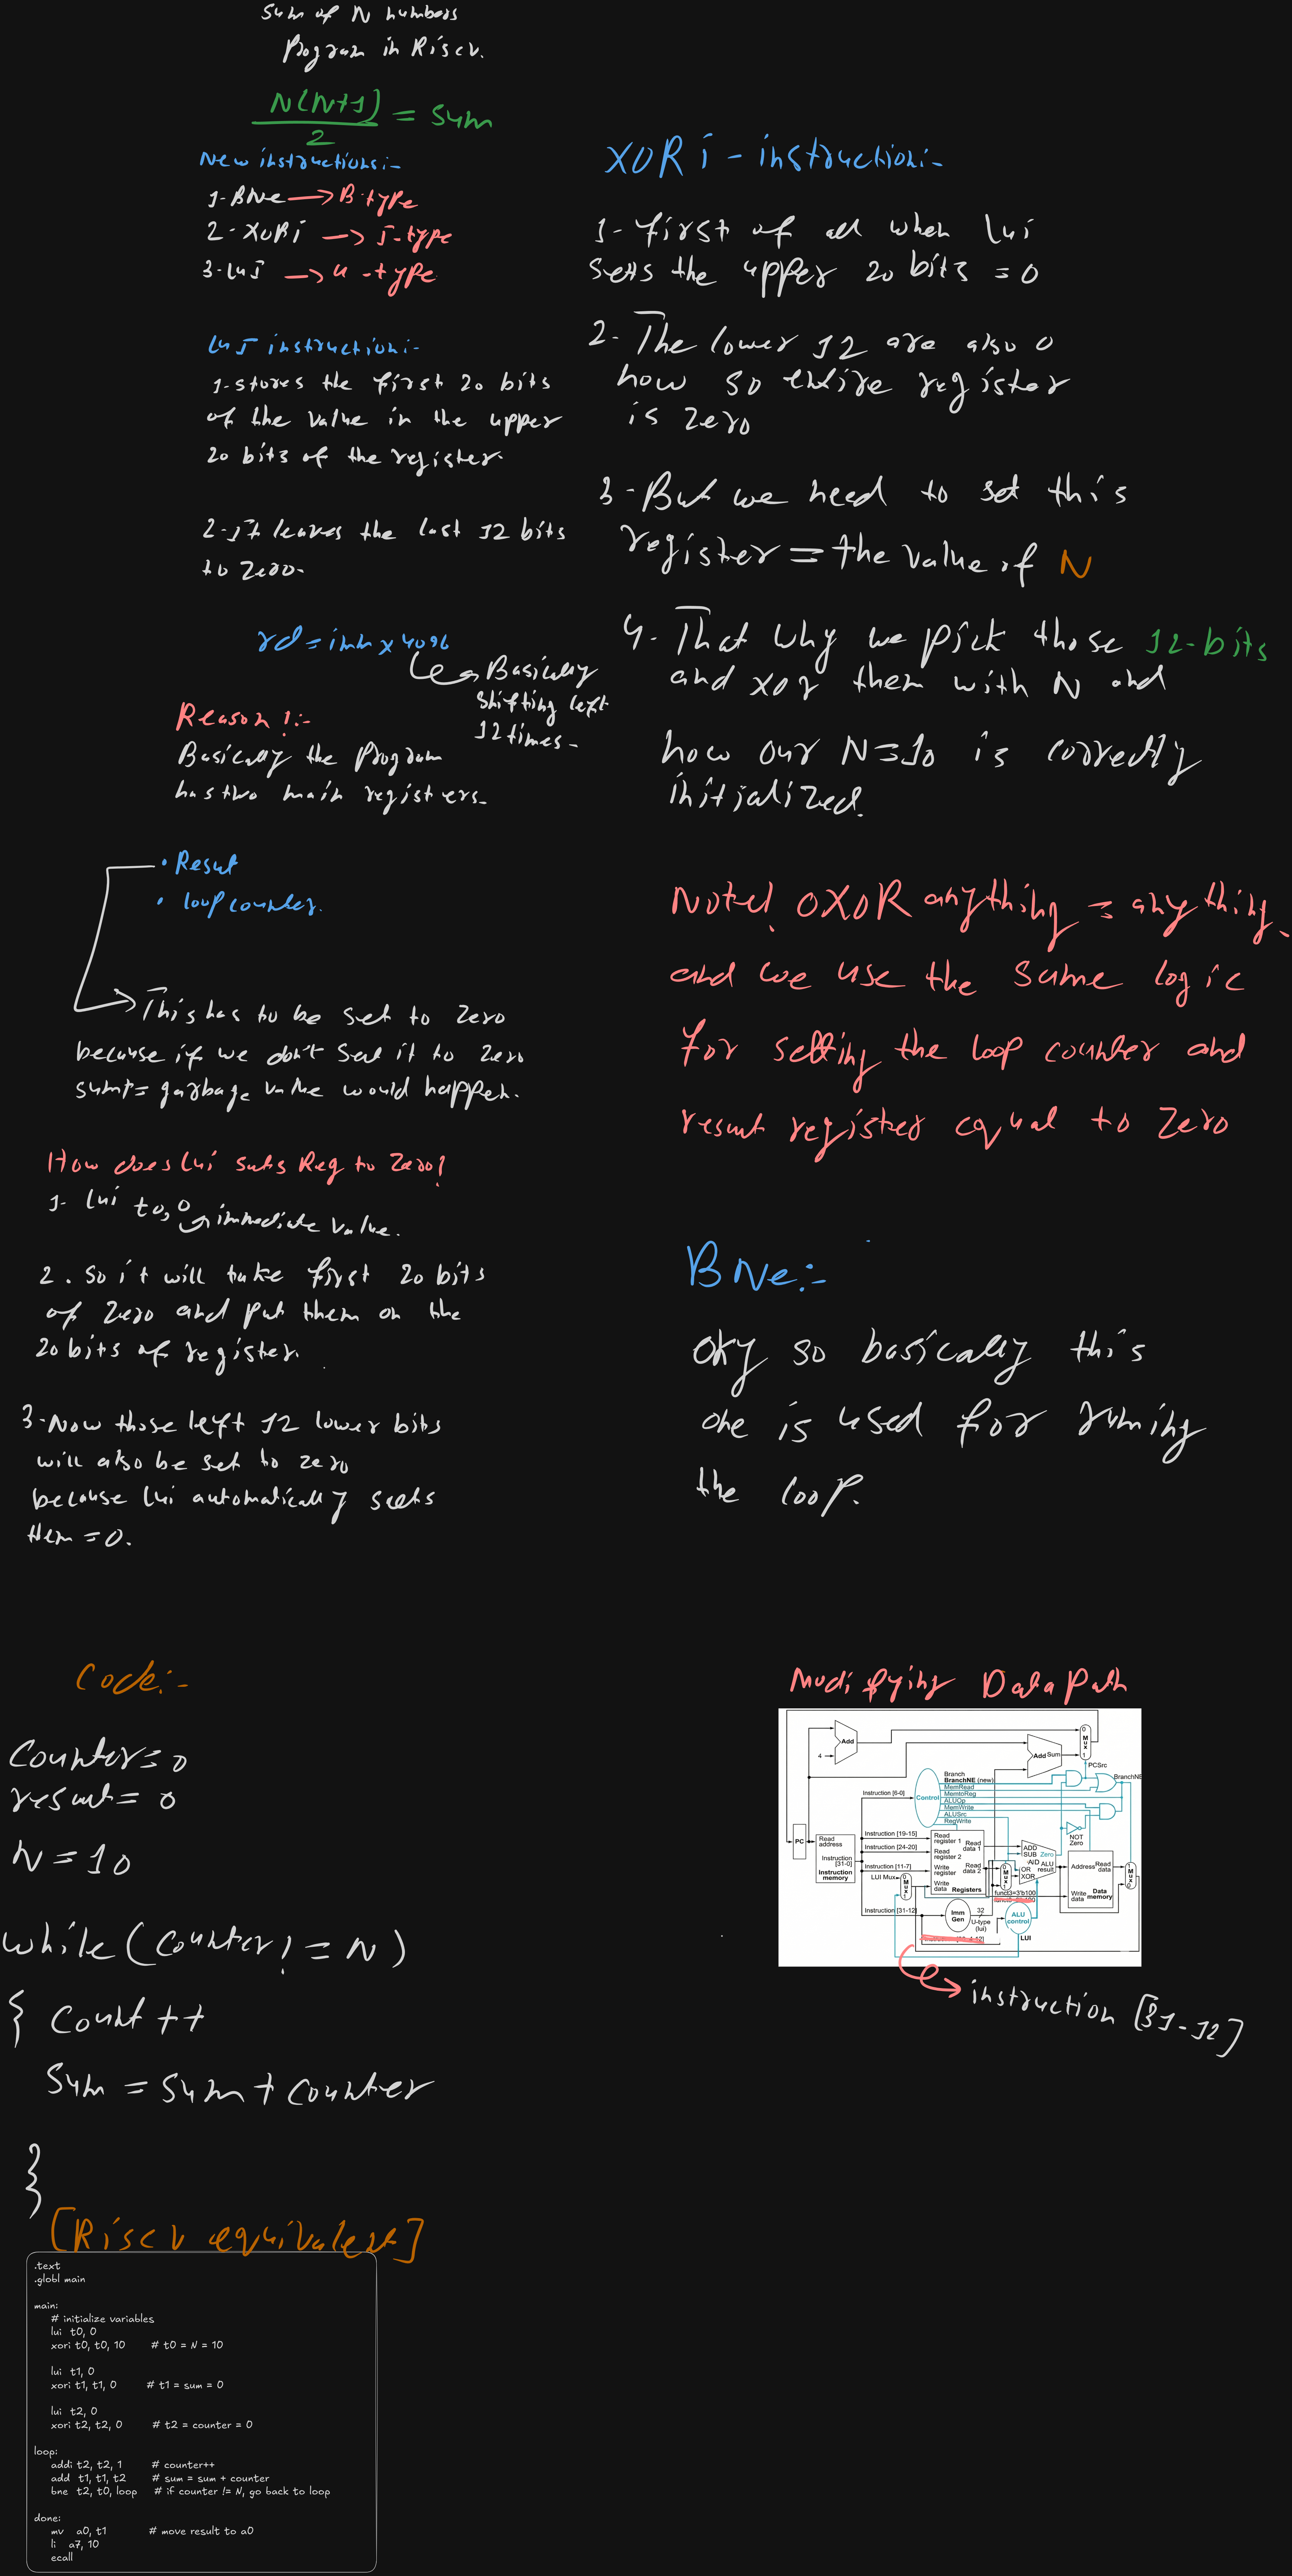
\includegraphics[height=0.82\textheight]{brainstorming-notes.png}
\caption{Design brainstorming: instruction selection rationale, LUI/XORI analysis, pseudocode for the summation loop, and datapath modifications.}
\end{figure}

\end{document}
